\documentclass[UTF8]{ctexart}

\usepackage{amsmath}
\usepackage{cases}
\usepackage{cite}
\usepackage{graphicx}
\usepackage[margin=1in]{geometry}
\geometry{a4paper}
\usepackage{fancyhdr}
\pagestyle{fancy}
\fancyhf{}


\title{基础物理实验报告}
\author{\LaTeX\ by\ 驰雨Chiyuru}
\date{\today}
\pagenumbering{arabic}

\begin{document}

\fancyhead[L]{驰雨Chiyuru}
\fancyhead[C]{弦振动实验}
\fancyfoot[C]{\thepage}

\maketitle
\tableofcontents
\newpage

\section{摘要}
本实验的原理为熟知的物理概念,意图使我们熟悉实验测量、数据处理和不确定度评估方法。实验通过测量数据和最小二乘法直线拟合得到劲度系数及其不确定度。通过分析误差来源和实验问题并对周期公式进行修正后,两种方法得到的劲度系数很好地符合。\cite{王合英2018自主探究实验对学生综合素质和创新能力的培养}


\section{实验仪器}
本实验的主要仪器为波尔共振仪和波耳共振仪控制箱。

\subsection{波尔共振仪}
波耳共振仪结构如图$1$所示。圆形摆轮$A$与弹簧$B$连接,构成待测振动系统。弹簧的另一端固定在摇杆$M$上的点$15$位置。摆轮边沿有一圈周期为$2$度的槽形缺口,光电门$H$通过测定缺口移动的个数来记录振动的幅度。


\subsection{波尔共振仪控制箱}
波尔共振仪控制箱使用方法可参考说明书。


\section{实验原理}

\subsection{弦振动方程}
一根柔软均匀的弦线两端被拉紧时,加以初始激励后由于弦线上的张力作用,弦线上的每一段带动邻段,振动传播到整条弦上。考察长度为$dx$的一段弦线的振动情况,利用牛顿第二定律在无位移的水平方向和有位移的竖直方向分别列出以下方程:

\begin{center}
    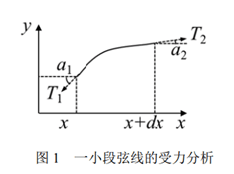
\includegraphics{picture/example.png}
\end{center}

\begin{numcases}{}
    T_2cos\alpha_2 - T_1cos\alpha_1 = 0 \\
    T_2sin\alpha_2 - T_1sin\alpha_1 = \rho dx\frac{\partial^2y }{\partial x^2} 
\end{numcases}

\subsection{弦线末端固定时的边界条件和振动的反射现象}
弦线末端固定时,振动脉冲在弦线上向末端传播并在末端发生反射。由弦振动方程可知,入射波波形为$y^+=f(vt+x)$,反射波波形为$y^-=f(vt-x)$。

\subsection{弦线在周期性正弦激励下的受迫振动和共振现象}
不想写了 qwq


\section{实验过程与数据分析}
\subsection{测量空气芯线圈与铝芯线圈的电阻与电感}
\subsubsection{$a. $计算出线圈$1$的电阻$R_1$和电感$L_1$}
在面包板上将L1的两端串联进初级电路中与电源和电阻板相连,将$L_2$的两端串联进次级电路,分别将万用表接在$L_1$,$L_2$,电源和电阻板的两端测量电压值并记录。\cite{王合英2008磁控溅射镀膜过程中非均匀磁场中电子的运动}
\subsubsection{$b. $确定线圈2的电阻$R_2$和电感$L_2$}
编不下去了。
\subsubsection{$c. $测量出带铝芯的线圈1的电阻$R_1^*$和电感$L_1^*$}
实验得到的数据如下:

\begin{center}
\begin{tabular}{|c|c|c|c|c|c|}
 \hline
线圈名称 & R'(Ω) & Va(V) & V(V) & Vr'(V) & Vo(V)\\
 \hline
线圈1(空气芯) & 560 & 6.733 & 4.52 & 4.568 & 3.925\\
 \hline
线圈2(空气芯) & 650 & 6.771 & 4.592 & 4.549 & 3.45 \\
 \hline
线圈3(铝芯) & 520 & 6.682 & 4.255 & 4.393 & 3.261\\
 \hline
线圈4(铝芯) & 510 & 6.685 & 4.286 & 4.113 & 3.151 \\
 \hline
\end{tabular}
\end{center}

\subsection{这里展示一下行间公式吧}
\subsubsection{行间公式}
% 行间公式用 $$ $$ 或者 \[ \] 来框住都可以,但在 LaTeX 中前者会改变行文的默认行间距,因此不推荐采用。
\paragraph{}这是一个不确定度计算。
\[
U_k=tinv(1-0.95,5-2)×s_k=0.752061
\]
\subsubsection{相对于行内公式}
这是一个不确定度计算:$U_k=tinv(1-0.95,5-2)×s_k=0.752061$


\section{分析与讨论}

\subsection{误差分析}

\subsubsection{实验中的系统误差}
来自万用表的精度影响。

受空间内电流与磁场的干扰。

\subsubsection{实验中的偶然误差}
接线时可能有未接触实的情况,导致接触电阻变大。面包板上的一些插孔较松,接线时有接触不良的问题存在,经反复调整后得以正常测量。

\subsection{实验后的思考}
本实验研究弦振动的多个参数之间的关系,这是一个多因素问题。在设计实验表格时我尝试了设计正交实验的方法,对各因素足够多的组合情形作研究,以求提高实验效率,均衡实验条件,简化计算过程和提高结果准确性。

\newpage
%图一般很大,建议换页。
\section{原始数据}
\begin{center}
    我随便插个图,各位自行修改。
    
    
    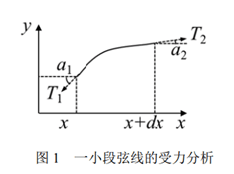
\includegraphics{picture/example.png}
\end{center}



\bibliographystyle{plain}

\bibliography{./template}  %bib文件名


\end{document}
